\documentclass{standalone}
\usepackage{hsbcommon}
%% Show/hide steps for standalone work — edit this line:
\makeatletter\AtBeginDocument{\@buildstepset{2,3}}\makeatother
\begin{document}
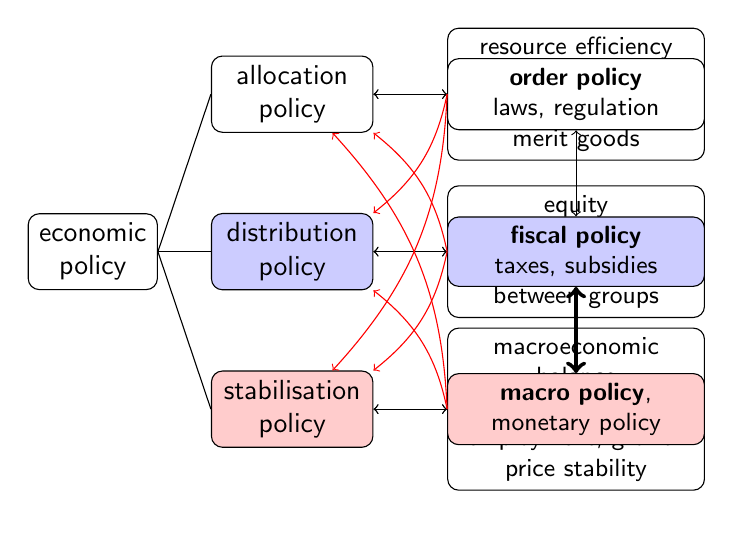
\begin{tikzpicture}
    \tikzset{
        every node/.style={
            draw,
            rounded corners,
            % text width=14ex,
            font=\sffamily
        }
    }
    \node[text width=width("economic"), align=center]  (ep) at (0.5,-2) {economic policy};
    \foreach[count=\i] \mypol/\mycom/\mycol in {
        allocation\\ policy/resource efficiency\\ market failures\\ public goods\\ merit goods/white,
        distribution\\ policy/equity\\ income and wealth\\ fairness and justice\\ between groups/blue,
        stabilisation\\ policy/macroeconomic balance\\ crisis prevention\\ high employment\\ growth\\ price stability/red%
    }{
        \node[anchor=west, text width=12ex,align=center,fill=\mycol!20]  (P\i) at (2,2-2*\i) {\mypol};
        \draw (ep.east) -- (P\i.west);
        \phantom{\node[anchor=west, text width=20ex, font=\small\sffamily,align=center] at (5,2-2*\i) (E\i)  {\mycom};}
        % \draw[<->] (P\i.east) -- (E\i.west);
    }

    \ifstep{1}{%%% explanations
    
        \foreach[count=\i] \mypol/\mycom/\mycol in {
            allocation\\ policy/resource efficiency\\ market failures\\ public goods\\ merit goods/white,
            distribution\\ policy/equity\\ income and wealth\\ fairness and justice\\ between groups/blue,
            stabilisation\\ policy/macroeconomic balance\\ crisis prevention\\ employment{,} growth\\ price stability/red%
        }{
            % \node[anchor=west, text width=12ex,align=center,fill=\mycol!20]  (P\i) at (2,2-2*\i) {\mypol};
            % \draw (ep.east) -- (P\i.west);
            \node[anchor=west, text width=20ex, font=\small\sffamily,align=center] at (5,2-2*\i) (E\i)  {\mycom};
            \draw[<->] (P\i.east) -- (E\i.west);
        }
    }
    \ifnotstep{1}
    {\ifstep{2}{%%% tools
    
        \foreach[count=\i] \mypol/\mycom/\mycol in {
            allocation/\textbf{order policy}\\ laws{,} regulation/white,
            distribution/\textbf{fiscal policy}\\ taxes{,} subsidies/blue,
            stabilisation/\textbf{macro policy}{,} monetary policy/red%
        }{
            % \node[anchor=west, text width=12ex,align=center,fill=\mycol!20]  (P\i) at (2,2-2*\i) {\mypol};
            % \draw (ep.east) -- (P\i.west);
            \node[fill=\mycol!20,anchor=west, text width=20ex, font=\small\sffamily,align=center] at (5,2-2*\i) (F\i)  {\mycom};
            \draw[<->] (P\i.east) -- (F\i.west);
        }
        \begin{scope}[red]
            \draw[->,bend left=20] (F1.west) to (P2);
            \draw[->,bend left=20] (F1.west) to (P3);
            \draw[->,bend right=20] (F2.west) to (P1);
            \draw[->,bend left=20] (F2.west) to (P3);
            \draw[->,bend right=20] (F3.west) to (P1);
            \draw[->,bend right=20] (F3.west) to (P2);
        \end{scope}
        \draw[<->] (F1) -- (F2);
        \draw[ultra thick,<->] (F2) -- (F3);
    }
    }

\end{tikzpicture}
\end{document}